% Don't touch this %%%%%%%%%%%%%%%%%%%%%%%%%%%%%%%%%%%%%%%%%%%
\documentclass[12pt]{article}
\usepackage{fullpage}
\usepackage[left=1in,top=1in,right=1in,bottom=1in,headheight=3ex,headsep=3ex]{geometry}
\usepackage{graphicx}
\usepackage{float}
\usepackage{array}


\newcommand{\blankline}{\quad\pagebreak[2]}
%%%%%%%%%%%%%%%%%%%%%%%%%%%%%%%%%%%%%%%%%%%%%%%%%%%%%%%%%%%%%%

% Modify Course title, instructor name, semester here %%%%%%%%

\title{PHY250 - Fall 2021: Review II}
\author{}
\date{}

%%%%%%%%%%%%%%%%%%%%%%%%%%%%%%%%%%%%%%%%%%%%%%%%%%%%%%%%%%%%%%

% Don't touch this %%%%%%%%%%%%%%%%%%%%%%%%%%%%%%%%%%%%%%%%%%%
\usepackage[sc]{mathpazo}
%\linespread{1.05} % Palatino needs more leading (space between lines)
\usepackage[T1]{fontenc}
\usepackage[mmddyyyy]{datetime}% http://ctan.org/pkg/datetime
\usepackage{advdate}% http://ctan.org/pkg/advdate
\newdateformat{syldate}{\twodigit{\THEMONTH}/\twodigit{\THEDAY}}
\newsavebox{\MONDAY}\savebox{\MONDAY}{Mon}% Mon
\newcommand{\week}[1]{%
%  \cleardate{mydate}% Clear date
% \newdate{mydate}{\the\day}{\the\month}{\the\year}% Store date
  \paragraph*{\kern-2ex\quad #1, \syldate{\today} - \AdvanceDate[4]\syldate{\today}:}% Set heading  \quad #1
%  \setbox1=\hbox{\shortdayofweekname{\getdateday{mydate}}{\getdatemonth{mydate}}{\getdateyear{mydate}}}%
  \ifdim\wd1=\wd\MONDAY
    \AdvanceDate[7]
  \else
    \AdvanceDate[7]
  \fi%
}
%\usepackage{setspace}
\usepackage{multicol}
%\usepackage{indentfirst}
\usepackage{fancyhdr,lastpage}
\usepackage{url}
\pagestyle{fancy}
\usepackage{hyperref}
\usepackage{lastpage}
\usepackage{amsmath}
\usepackage{layout}

\lhead{}
\chead{}
%%%%%%%%%%%%%%%%%%%%%%%%%%%%%%%%%%%%%%%%%%%%%%%%%%%%%%%%%%%%%%

% Modify header here %%%%%%%%%%%%%%%%%%%%%%%%%%%%%%%%%%%%%%%%%
%\rhead{\footnotesize Text in header}

%%%%%%%%%%%%%%%%%%%%%%%%%%%%%%%%%%%%%%%%%%%%%%%%%%%%%%%%%%%%%%
% Don't touch this %%%%%%%%%%%%%%%%%%%%%%%%%%%%%%%%%%%%%%%%%%%
\lfoot{}
\cfoot{\small \thepage/\pageref*{LastPage}}
\rfoot{}

\usepackage{array, xcolor}
\usepackage{color,hyperref}
\definecolor{clemsonorange}{HTML}{EA6A20}
\hypersetup{colorlinks,breaklinks,linkcolor=clemsonorange,urlcolor=clemsonorange,anchorcolor=clemsonorange,citecolor=black}

\begin{document}

\maketitle




% First Section %%%%%%%%%%%%%%%%%%%%%%%%%%%%%%%%%%%%%%%%%%%%


\newcounter{example}
\setcounter{example}{1}
\section*{Exercise \theexample}

A block with mass M rests on a frictionless surface
and is connected to a horizontal spring of force constant k. The
other end of the spring is attached to a wall (Fig. P14.72). Asecond
block with mass m rests on top of the first block. The coefficient of
static friction between the blocks is$\mu_s$. Find the maximum amplitude
of oscillation such that the top block will not slip on the bottom
block.

\begin{figure}[h!]
  \begin{center}
    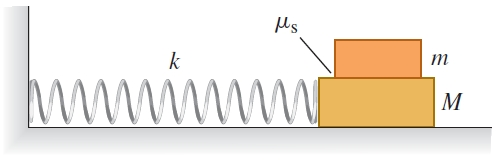
\includegraphics[height=1.in]{images/4.jpg}
  \end{center}
\end{figure}

% First Section %%%%%%%%%%%%%%%%%%%%%%%%%%%%%%%%%%%%%%%%%%%%

\stepcounter{example}
\section*{Exercise \theexample}


A square object of
mass m is constructed of four
identical uniform thin sticks, each
of length L, attached together.
This object is hung on a hook
at its upper corner.
If it is rotated slightly to the
left and then released, at what
frequency will it swing back and
forth?

\begin{figure}[h!]
  \begin{center}
    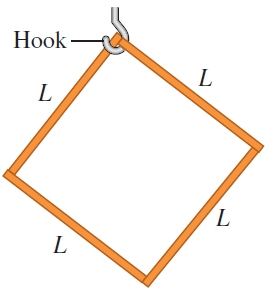
\includegraphics[height=2.in]{images/3.jpg}
  \end{center}
\end{figure}


% First Section %%%%%%%%%%%%%%%%%%%%%%%%%%%%%%%%%%%%%%%%%%%%

\stepcounter{example}
\section*{Exercise \theexample}

A $5.00$-m, $0.732$-kg wire is used to support two uniform
235-N posts of equal length (Fig. P15.62). Assume that the
wire is essentially horizontal and that the speed of sound is $344$ m/s
A strong wind is blowing, causing the wire to vibrate in
its 5th overtone. What are the frequency and wavelength of the
sound this wire produces?

\vspace{5mm}

 \begin{figure}[h!]
  \begin{center}
    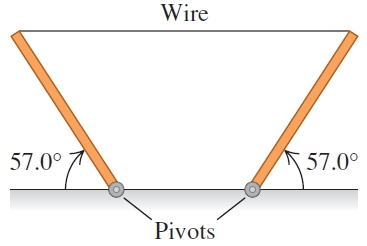
\includegraphics[height=1.5in]{images/1.jpg}
  \end{center}
\end{figure}


% First Section %%%%%%%%%%%%%%%%%%%%%%%%%%%%%%%%%%%%%%%%%%%%

% \stepcounter{example}

% \section*{Exercise \theexample}
% A long spring
% such as a Slinky™ is often used to demonstrate longitudinal
% waves. (a) Show that if a spring that obeys Hooke’s law has mass
% m, length L, and force constant $k'$ the speed of longitudinal waves
% on the spring is $v=L\sqrt{k'/m}$. (b) Evaluate
% for a spring with m = 0.250 kg, L = 2.00 m, and $k'$ = 1.50 N/m.

% First Section %%%%%%%%%%%%%%%%%%%%%%%%%%%%%%%%%%%%%%%%%%%%

\stepcounter{example}

\section*{Exercise \theexample}


The gas cloud known as the Crab Nebula
can be seen with even a small telescope. It is the remnant of a
supernova, a cataclysmic explosion of a star. The explosion was
seen on the earth on July 4, 1054 C.E. The streamers glow with the
characteristic red color of heated hydrogen gas. In a laboratory on
the earth, heated hydrogen produces red light with frequency $4.568\times10^{14}~$Hz;
the red light received from streamers in the
Crab Nebula pointed toward the earth has frequency $4.586\times10^{14}~$Hz.
(a) Estimate the speed with which the outer edges of the
Crab Nebula are expanding. Assume that the speed of the center of
the nebula relative to the earth is negligible. ( The speed of light is $3\times10^8$ m/s
). (b) Assuming that the expansion speed has been
constant since the supernova explosion, estimate the diameter of
the Crab Nebula. Give your answer in meters and in light-years.
(c) The angular diameter of the Crab Nebula as seen from earth is
about 5 arc minutes (1 arc minute=$1/60$ degree). Estimate the distance
(in light-years) to the Crab Nebula, and estimate the year in
which the supernova explosion actually took place.




% First Section %%%%%%%%%%%%%%%%%%%%%%%%%%%%%%%%%%%%%%%%%%%%

\stepcounter{example}

\section*{Exercise \theexample}

Two identical loudspeakers
are located at points $A$
and $B$, $2.00$ m apart. The loudspeakers
are driven by the same
amplifier and produce sound
waves with a frequency of $784$
Hz. Take the speed of sound in
air to be $344$ m/s. A small
microphone is moved out from
point B along a line perpendicular
to the line connecting A and
B . (a)
At what distances from B will there be destructive interference?
(b) At what distances from B will there be constructive interference?
(c) If the frequency is made low enough, there will be no
positions along the line BC at which destructive interference
occurs. How low must the frequency be for this to be the case?
\vspace{5mm}

 \begin{figure}[h!]
  \begin{center}
    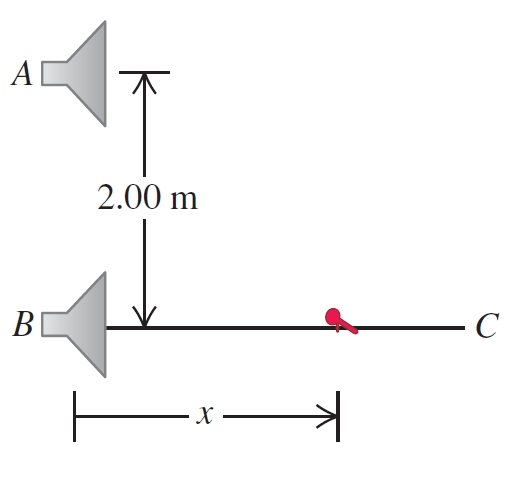
\includegraphics[height=2.5in]{images/2.jpg}
  \end{center}
\end{figure}






\end{document}


